% $Id: Field_usage.tex,v 1.4 2003/12/17 20:20:26 svasquez Exp $

%\subsection{Design}

% <Describe strategy for overall class design.>


The Field class aggregates two internal subclasses: a GlobalField class
and a LocalField class.  This separation allows the code to clearly
differentiate between functions which operate internal to a single DE
on a local decomposition of data, 
and those which must be aware of the
global state of the Field.  
 
There is a correspondence between the Global Distributed Grid class,
and the Local Distributed Grid class, and Fields.  Each DE contains
the corresponding local decompositions for Distributed Grids and Fields.

The Field class maintains the relationship of
how data maps onto the grid (e.g. one item per cell located at
the cell center, one item per cell located at the NW corner, 
one item per cell vertex, etc).  This means that different Fields
which are on the same underlying Grid but have different
mappings (staggerings) can share the same Grid object without
needing to copy or replicate it multiple times.  Regridding
operations can operate first on the shared Grid, and then
use the staggering information from the Field to compute the
corresponding transformation of the data.

Some methods which have a Field interface will actually be
implemented at the underlying Grid or Array level; they
will be inherited by the Field class.  This allows the user
API (Application Programming Interface) to present functions at
the level which is most consistent to the application without
restricting where inside the ESMF the actual implementation
is done.

\input{../Infrastructure/Field/doc/ESMF_FieldCreateEx_fapi}

% cecelia - this is the new section on the data interfaces to the
% communications routines.  move it where you want.   nsc 31jul03

\subsection{Distributed Data Methods}

There are ten methods which involve movement of data between DEs.
The first three are higher level functions which are intended to
map closely to needs of applications programs.  They are:

\subsubsection{Halo}
% $Id: ArrayHalo_desc.tex,v 1.2 2003/11/14 20:52:23 jwolfe Exp $


Halo operations update ghost-cell or halo regions at the boundaries
of a local data decomposition.  Halo regions are to be considered
read-only by the local process; their data values can be used to
compute the new values for cells which are local to this process,
but they cannot be updated except by a Halo operation.




\subsubsection{Regrid}
% $Id: Regrid_usage.tex,v 1.8 2005/11/19 00:30:16 jwolfe Exp $


Regrid is designed to be called with Field or Bundle
arguments in order to utilize information embedded in
these objects.  For example, Regrid requires knowledge
of underlying grid information (both PhysGrid and DistGrid)
and of the relative location (staggering) of Fields on
the Grid.  In addition, Regrid uses any mask information
that may be associated with a Field.  However, ESMF also
provides an Array interface for users who have gathered all
necessary information.

Regrid is separated into RegridStore functions, a Regrid
function, and a RegridRelease function. The Store functions
compute interpolation weights and initialize communication
requirements for performing a regridding of a Field
from one Grid to another.  The Regrid function uses
a created Regrid object to perform the actual regridding
of Fields or Bundles.  The Release function deletes the
Regrid object and frees all memory associated with a Regrid.
The reason for the separation is that in many cases, the
initial creation is expensive and re-used often throughout
an application.  The Regrid and RegridRelease functions are
also common to all the Regrid methods.

Because many methods are supported for regridding,
the main Store function branches to a specific
creation function based on the regrid method requested
(e.g. bilinear, conservative, spectral).  Each of
these regrid methods are in a separate module to
prevent the main Regrid module from becoming too
large.  The user is unaware of this hierarchy as the
top-level module provides a unified API.

\subsubsection{Regrid and Grid Overlap}

Regrid assumes both the source and destination Grids share the same coordinate
system and units.  Although 3D regridding is not yet available, this rule is
also expected to be valid for vertical grids as well.  Users are responsible
for any necessary conversion or translation.

There are five possible physical overlap situations between the source and
destination Grids, illustrated in Figure \ref{fig:RegridGridOverlap}.

\begin{center}
\begin{figure}
\caption{Possible Relationships between Grids in Physical (Coordinate) Space. }
\label{fig:RegridGridOverlap}
\resizebox{\textwidth}{!}
  {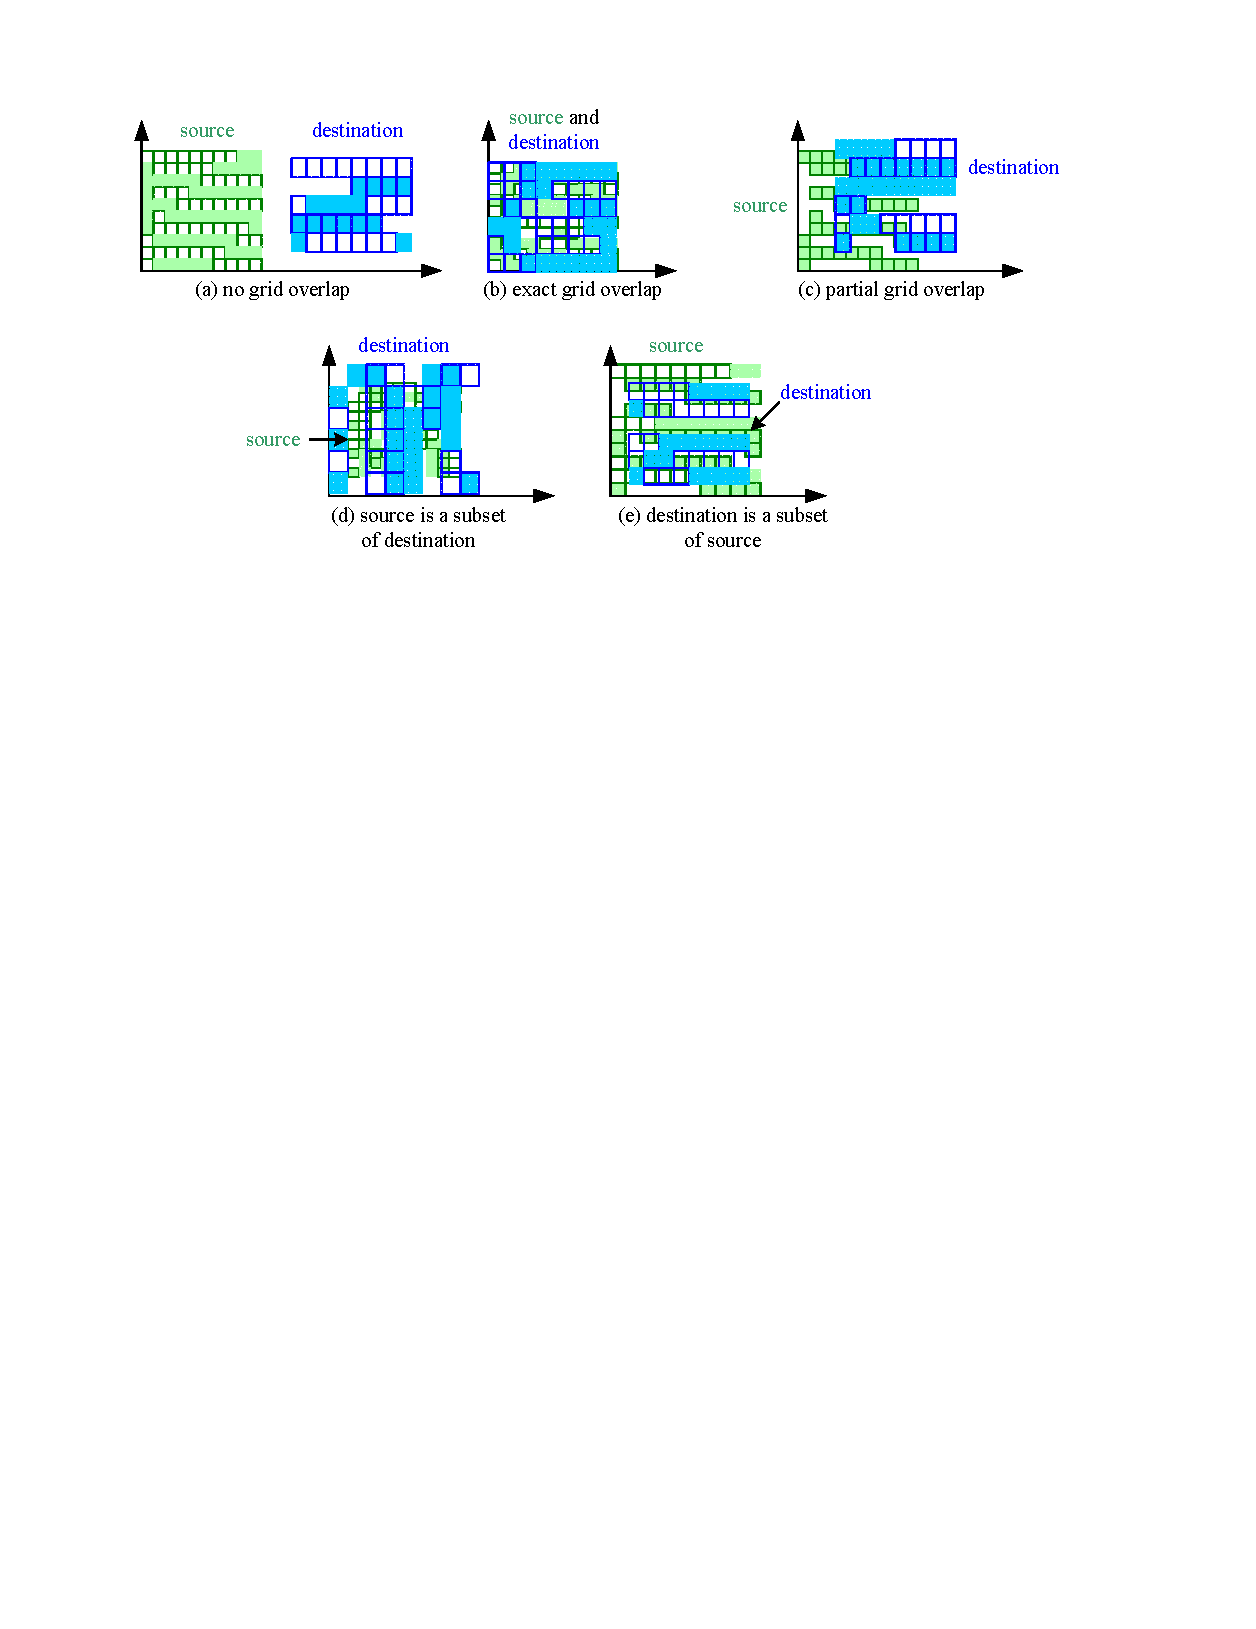
\includegraphics{RegridGridOverlap}}
\end{figure}
\end{center}

Regrid can provide complete interpolation weights for the destination Field
only for those situations where there is source data covering the entire physical
domain of the destination Grid (cases (b) and (e) above).  In all the other
cases, there are parts of the destination Grid for which there is no source. 
When source data is not available, Regrid routines will not extrapolate data
values and the destination Field may contain data points that have not been
calculated or filled.  Currently, regrid routines initialize the destination
Field to a value of zero prior to regridding, so unfilled destination data points
will have that value.  In the future, regrid routines will have an optional
argument allowing users to specify a fill value besides zero.  


\subsubsection{Regrid and Data Location}

There is no restriction in Regrid that the source and destination Fields
define their data in the same relative location (RelLoc).  However, regridding
between Fields with different RelLocs can have unintended consequences if the
related Grids cover exactly the same physical domain.  The RelLocs represent
different subGrids, which can shift the represented physical domain by plus or
minus one-half of a cell width.  This is illustrated below in Figure 
\ref{fig:RegridRelLocEffect}, which shows the physical areas described by two

\begin{center}
\begin{figure}
\caption{Illustration of Grid areas represented by differing RelLocs. }
\label{fig:RegridRelLocEffect}
\resizebox{\textwidth}{!}
  {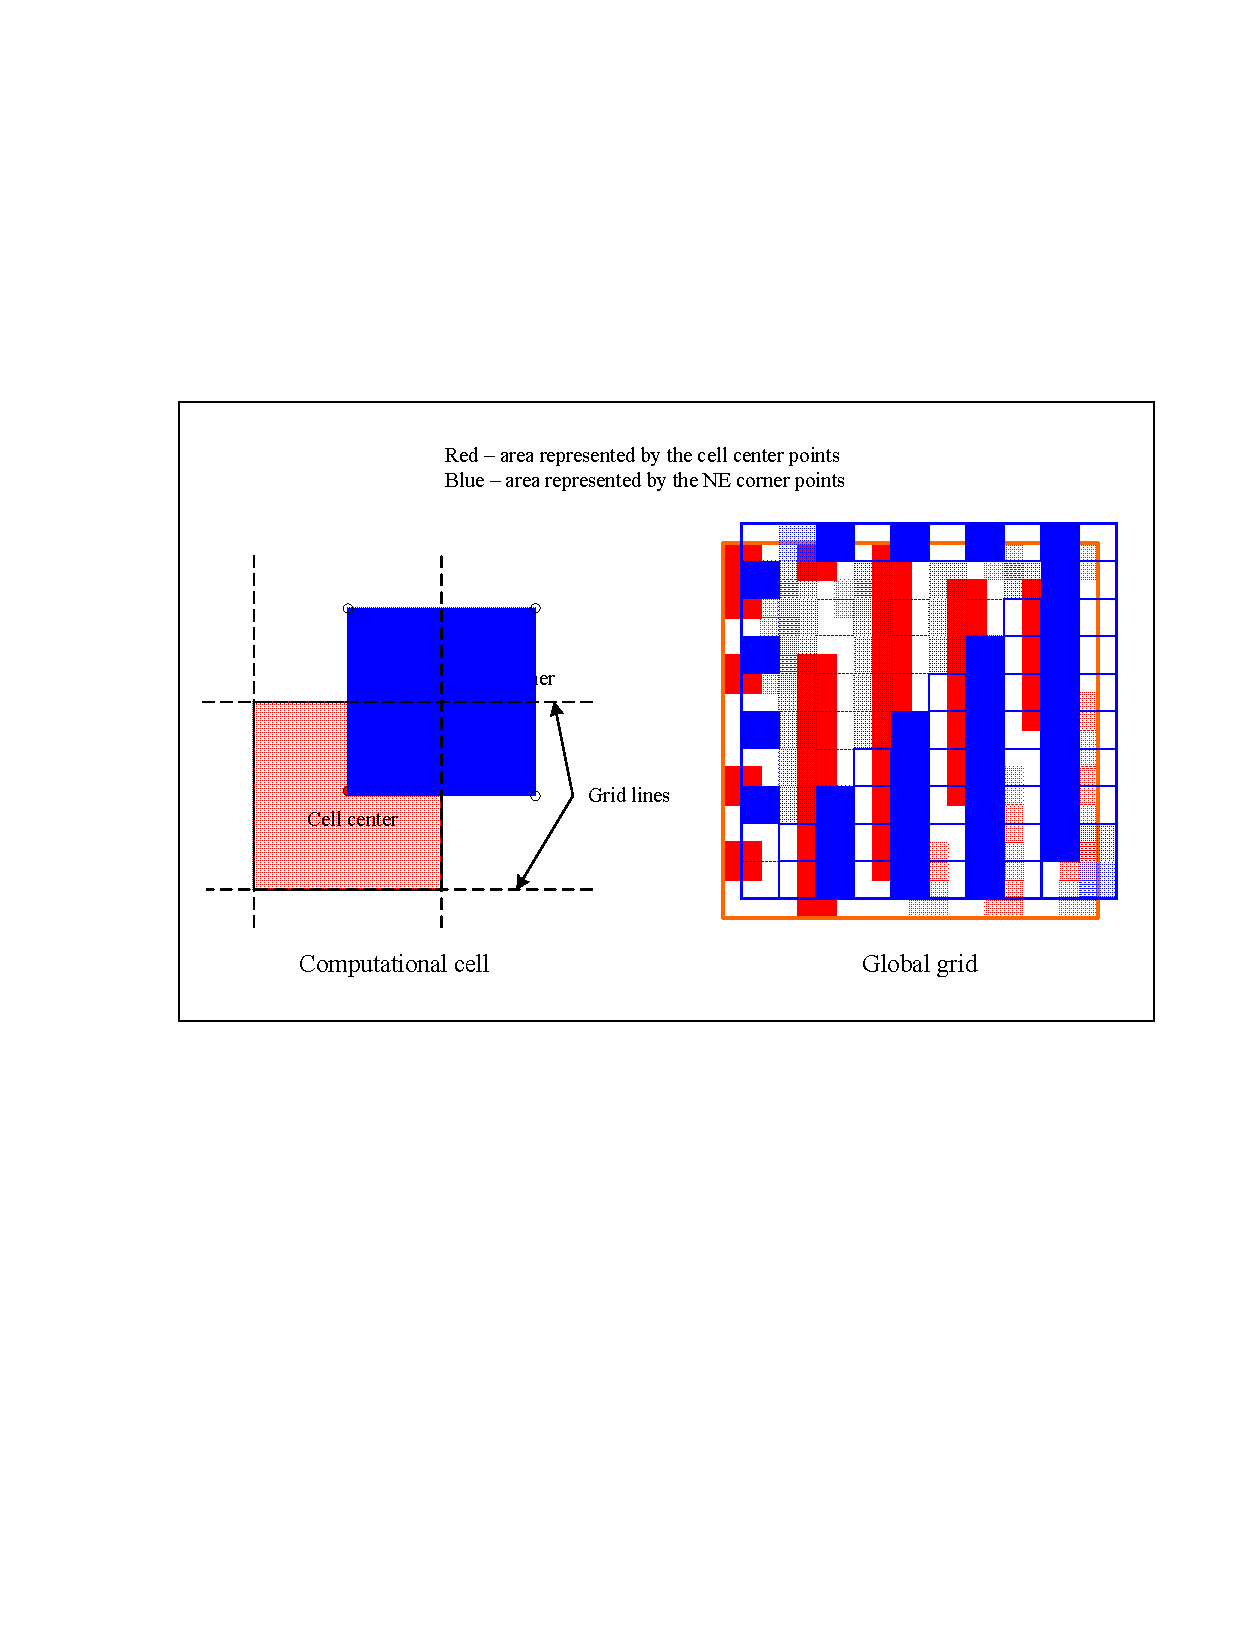
\includegraphics{RegridRelLocEffect}}
\end{figure}
\end{center}

sample RelLocs and the effect on the overlap of the global Grids.  In this
situation, there may be some unfilled or less accurate data at some of the
Grid boundaries.

Different refinement or cell sizes between the source and destination Grids
may also have a similar effect, even if their corresponding Fields have the
same RelLocs.  This is illustrated below...


\subsubsection{Regrid and Periodicity}





\subsubsection{Redist}
% $Id: ArrayRedist_desc.tex,v 1.3 2004/06/22 21:35:25 jwolfe Exp $


Redistribution operations always operate on data associated with a
single Grid, but are either decomposed across multiple processors
differently, or have different index orderings, or are decomposed
in different dimensions.  The Redistribution methods involve only
data movement; no interpolation, data binning, averaging, etc are
performed.  A typical example of Redistribution is the data transpose
associated with the translation between phycial and Fourier space.

An example of the use of ESMF Redistribution methods is presented in
the FieldRedist system test.

In the future, we plan to have specific interfaces for common uses
like the data transpose.


\subsubsection{Lower Level Functions}
The last seven correspond closely to the lower level
MPI communications primitives.  They are:
\begin{description}
\item[Gather]
Reassembling data which is decomposed over a set of DEs into a single
block of data on one DE.
\item[AllGather]
Reassembling data which is decomposed over a set of DEs into multiple
copies of a single block of data, one copy per original DE.
\item[Scatter]
Spreading an undecomposed block of data on one DE over a set of DEs,
decomposing that single block into smaller subsets of data, one
data decomposition per DE.
\item[AlltoAll]
Spreading an undecomposed block of data from multiple DEs onto
each of the other DEs in the set, resulting in a set of multiple decomposed 
data blocks per DE, one from each of the original source DEs.
\item[Broadcast]
Spreading an undecomposed block of data from one DE onto all other
DEs, where the resulting data is still undecomposed and simply
copied to all other DEs.
\item[Reduction]
Computing a single data value, e.g. the data maximum, minimum, sum, etc
from a group of decomposed data blocks across a set of DEs, where the
result is delivered to a single DE.
\item[AllReduce]
Computing a single data value, e.g. the data maximum, minimum, sum, etc
from a group of decomposed data blocks across a set of DEs, where the
result is delivered to all DEs in the set.
\end{description}

Each of these methods can be called on Bundles, with and without packed
data, on Fields, and on Arrays.

